\documentclass[6pt,twoside]{article}
\usepackage{amsmath, setspace,enumitem, graphicx ,amssymb,amsthm,epsfig,epstopdf,titling,url,array, caption, cite, hyperref}
\graphicspath{ {C:/Users/mburanos/Downloads/}}

\renewcommand{\labelenumii}{\theenumii}
\renewcommand{\theenumii}{\theenumi.\arabic{enumii}.}

\DeclareCaptionType{code}[Example][List of Examples]
\theoremstyle{plain}
\theoremstyle{definition}
\newtheorem{defn}{Definition}[section]
\newtheorem{thm}{Theorem}[section]

\renewcommand{\baselinestretch}{1.2} 

\title{FDTool: a Python application to mine for functional dependencies and candidate keys in tabular data}
\author{Matt Buranosky, \\
Elmar Stellnberger, \\
Emily Pfaff, \\
Cavin Ward-Caviness}
\date{\today}

\begin{document}
\maketitle
\begin{abstract}
Functional dependencies and candidate keys crucially serve in the process of table decomposition, database  normalization, and data cleansing. In this paper, we present FDTool, a command line Python application to discover functional dependencies in tabular datasets and infer equivalences and candidate keys from them. 

\bigskip
\noindent
We are working out of  \textbf{https://github.com/USEPA/FDTool}.
\end{abstract}

\begin{section}{Functional Dependencies}

Functional dependencies (FDs) are researched to better understand how attributes in a database schema relate to one another. An FD defines a rule constraint between two sets of attributes in a relation $r(U)$, where $U = \{ v_1, v_2, \ldots, v_m \}$ is a finite set of attributes. A combination of attributes over a dataset is called a \textit{candidate}. An FD $X \rightarrow Y$ asserts that the values of candidate $X$ uniquely determine those of candidate $Y$. For example, the social security number (SSN) attribute in a dataset of public records functionally determines the first name attribute; we write $\{SSN\} \rightarrow \{first\text{\_}name\}$.

\begin{defn}
A \textit{functional dependency} $X \rightarrow Y$, where $X, Y \subseteq U$, is satisfied by $r(U)$, if for all pairs of tuples $t_i, t_j \in r(U)$, we have that $t_i\left[X\right]=t_j\left[X\right] \  \text{implies} \ t_i\left[Y\right]=t_j\left[Y\right]$. 
\end{defn}

 In this case, $X$ is the \textit{left hand side} of an FD, and $Y$ is the \textit{right hand side}. If $Y$ is not functionally dependent on any proper subset of $X$, then $X \rightarrow Y$ is \textit{minimal}. Minimal FDs are our only concern in rule mining FDs, since all other FDs are logically implied. For instance, if we know $\{SSN\} \rightarrow \{first\text{\_}name\}$, then we can infer that $\{SSN,\  last\text{\_}name\} \rightarrow \{first\text{\_}name\}$. 

\subsection[Power set lattice]{Power set lattice}

The search space for FDs is represented as a \textit{power set lattice} of nonempty attribute combinations.

\begin{figure}[h]
	\centering
	\fbox{\includegraphics[width=0.65\columnwidth, height=5cm]{LatticeABCD}}
	\textbf{\label{Fig. 1}}
	\caption{Nonempty combinations of attributes $A$, $B$, $C$, and $D$ by k-level.}
	\label{fig:lattice}
\end{figure}

Figure \ref{fig:lattice} gives the nonempty combinations of attributes of a relation $r(U)$ such that $U = \{ A, B, C, D\}$. There are $2^{n} - 1 = 2^{4} - 1 = 15$ attribute subsets in the power set lattice. Each combination $X$ of the attributes in $U$ can be the left hand side of an FD $X \rightarrow Y$ such that $X \rightarrow Y$ is satisfied by relation $r(U)$. Since the attribute set itself $U$ trivially determines every one of its subsets, it can be ignored as a candidate. There remain $2^{n}-2 = 2^{4} - 2 = 14$ nonempty, proper subsets of $U$ that are to be considered candidates.

There are $n \cdot 2^{n-1}-n=4 \cdot 2^{4-1}-4 = 28$ edges (or arrows) in the semi-lattice of the complete search space for FDs in relation $r(U)$. The size of the search space for FDs is exponentially related to the number of attributes in $U$. Hence, the search space for FDs increases quite significantly with a greater number of attributes in $U$. For instance, when there are $10$ attributes in a relation, the search space for FDs climbs to $5110$. This gives reason to be cautious of runtime and memory costs when deploying a rule mining algorithm to discover FDs.


\subsection[Partition]{Partition}

The algorithms used to discover FDs differ in their approach to navigating the complete search space of a relation. Their candidate pruning methods vary and sometimes the methods used to validate FDs do as well. These discrepancies competitively affect runtime and memory behavior when used to process tables of different shapes. 

The most common data structure used to validate FDs is the partition. A partition places tuples that have the same values on an attribute into the same group. 

\begin{defn}
	\label{partition}
	Let $X \subseteq U$ and let $t_1, \ldots , t_n$ be all the tuples in a relation $r(U)$. The \textit{partition} over $X$, denoted $\prod_X$, is a set of the groups such that $t_i$ and $t_j$, $1 \leq i$, $j \leq n$, $i \neq j$, are in the same group if and only if $t_i\left[X\right]=t_j\left[X\right]$.
\end{defn}

It follows from Definition \ref{partition} that the \textit{cardinality of the partition} $\mathbf{card}(\prod_{A} (r))$ is the number of groups in partition $\prod_{A}$. The cardinality of the partition offers a fast approach to validating FDs in a dataset.

\begin{thm}
	\label{valFD}
	An FD $X \rightarrow Y$ is satisfied by a relation $r(U)$ if and only if $\mathbf{card}(\prod_X) = \mathbf{card}(\prod_{XY})$.
\end{thm}

Theorem \ref{valFD} provides an efficient method to check whether an FD $X \rightarrow Y$ holds in a relation. \footnote{FDTool uses Theorem \ref{valFD} as means to check FDs in the GetFDs module with the \textit{pandas} data analysis library functions \textit{nunique()} and \textit{dropduplicates.count()}.}

\subsection[closure]{Closure}

Efforts in relational database theory have lead to more runtime and memory efficient methods to check the complete search space of a relation for FDs. In place of needing each arrow in a semi-lattice checked, we can infer the FDs that logically follow from those already discovered. Such FDs are to be discovered as a consequence of \textit{Armstrong`s Axioms}, which are as follows: \textit{Reflexivity}: $Y \subseteq X$ implies $X \rightarrow Y$; \textit{Augmentation}: $X \rightarrow Y$ implies $XZ \rightarrow YZ$; \textit{Transitivity
}: $ X \rightarrow Y$ and $Y \rightarrow Z$ imply $X \rightarrow Y$. 

These axioms signal the distinction between FDs that can be inferred from already discovered FDs, and those that cannot (Maier 1983). Exploiting Armstrong's Axioms allows us to avoid having to check as many candidates on the right hand side of FDs.

\begin{defn}
	\label{closure}
	Let $F$ be a set of functional dependencies over a dataset $D$ and $X$ be a candidate over $D$. The \textit{closure of candidate} $X$ with respect to $F$, denoted $X^{+}$, is defined as $ \left\{  Y \ | \  X \rightarrow Y \  \text{can be deduced from} \ F \ \text{by Armstrong's Axioms} \right\}$.
\end{defn}

The \textit{nontrivial closure of candidate} $X$ with respect to $F$ is defined as $X^{*} = X^{+} \setminus X$ and written $X^{*}$. \footnote{FDTool saves the closure of candidates at each level before releasing it from memory at levels that follow.}

\end{section}

\begin{section}{Pruning Rules}

Existing functional dependency algorithms are split between three categories: \textit{Difference- and agree-set algorithms} (e.g., Dep-Miner, FastFDs), \textit{Dependency induction algorithms} (e.g., FDEP), and \textit{Lattice traversal algorithms} (e.g., TANE, FUN, FD\_Mine, DFD). 

\subsection[Lattice traversal algorithms]{Lattice traversal algorithms}

Lattice traversal algorithms model the search space of a relation as a power set lattice. Most of such algorithms, i.e., TANE, FUN, and FD\_Mine, use a level-wise approach to traversing the search space of a relation from the bottom-up. They start by checking for FDs that are singleton sets on the left hand side and iteratively transition to candidates of greater cardinality.

\begin{defn}
	\label{k-level}
	Let $X_{1}$, $X_{2}$, \ldots, $X_{k}$, $X_{k+1}$ be $(k+1)$ attributes over a database $D$. If $X_{1}X_{2}$ \ldots $X_{k} \rightarrow X_{k+1}$ is an FD with $k$ attributes on its left hand side, then it is called a \textit{k-level} FD. 
\end{defn}

The search space for FDs is reduced at the end of each iteration using pruning rules. \textit{Pruning rules} check the validity of candidates not yet checked with FDs already discvored and those inferred from Armstrong's Axioms. After a search space is pruned, an \textit{Apriori\_Gen} principle generates $k$-level candidates with the $(k-1)$-level candidates that were not pruned. \footnote{\textit{Apriori\_Gen} methods differ in approach across implementations. FDTool computes the power set of remaining $k$-level candidates and collects the members who share a cardinality of $k+1$.} Pruning reduces the number of candidates that are to be checked on the left hand side of FDs.

{\setstretch{1.0}
\bigskip
\noindent
\textbf{Apriori\_Gen}:

\begin{itemize}[leftmargin=*]
\item \textit{OneUp}: generates all possible candidates in $C_k$ from those in $C_{k-1}$.
\item \textit{OneDown}: generates all possible candidates in $C_{k-1}$ from those in $C_k$.
\end{itemize}
} 

Level-wise lattice traversal algorithms stop iterating after all candidates in a search space are pruned. In this case, \textit{Apriori\_Gen} generates the null set $\emptyset$ raising a flag for the algorithm to terminate. This has the effect of shortening runtime to the degree that FDs are discovered and others are inferred.

The level-wise lattice traversal algorithms, TANE, FUN, and FD\_Mine, differ in terms of pruning rules. TANE, for example, uses partitions to discover FDs. If the FD $AC \rightarrow B$ had been discovered, then $ACD \rightarrow B$ and $ACDE \rightarrow B$ are implied and need not be checked.

\subsection[FD\_Mine]{FD\_Mine}

FD\_Mine performs favorably to many other of such algorithms on relational database schemas made up of long and narrow tables, i.e., those with many rows and few columns ($\leq14$). This puts FD\_Mine in a special position to rule mine bioinformatics data consisting of long sets of patient records. 

\begin{defn}
	\label{eq}
	Let $X$ and $Y$ be candidates over a dataset $D$. If $X \rightarrow Y$ and $Y \rightarrow X$ hold, then we say that $X$ and $Y$ are an \textit{equivalence} and denote it as $X \leftrightarrow Y$. 
\end{defn}

Let $R$ be a relational schema and $X$ be a candidate of $R$ over a dataset $D$. If $X \cup X^{*} = R$, then $X$ is a \textit{key}.


\subsection[Non-minimal FDs]{Non-minimal FDs}

\bigskip
{\setstretch{1.0}
\noindent
\textbf{Prune}$\left( C_{k} \text{, } E \text{, } Closure \right)$ \footnote{Closure = $\left\{  X^{+} \ | \  X \in C_{k} \vee X \in OneDown \left[ C_{k} \right] \right\}$.}\footnote{Equivalent candidates are stored in $E$.}\footnote{All candidates at level $k$ are stored in $C_k$.}
\begin{tabbing}
 \hspace{30pt}\=\hspace{30pt}\=\hspace{30pt}\=\hspace{30pt}\=\kill
01 for each $S \in C_k$: \\
02	\> for each $X \in OneDown\left[  C_k \right]$: \\
03	\> \>  if $\left( X \subset S \right)$ then: \\
04	\> \> \> $S^{+} = S^{+}  \cup X^{*}$ \\
05	\> \> \> if $\left( X \in \left\{ Z \ | \ Y \leftrightarrow Z \in E \right\} \right)$ then: \\
06	\> \> \> \> delete $S$ from $C_k$ \\
07 	\> \> \> if $S \subset X^{+}$ then: \\
08 	\> \> \> \> delete $S$ from $C_k$ \\
09 	\> \> \> if $U == S^{+}$ then: \\
10 	\> \> \> \> delete $S$ from $C_k$ \\
11 return $C_k$, \textit{Closure};
\end{tabbing}
} 

\cite{expAlgs}
\cite{fdmine1}
\cite{fdmine2}
\cite{dbbook}

\end{section}

\begin{section}{Experimentation}

FDTool was initially created to help decompose datasets of medical records as part of the Clinical Archived Records Research for Environmental Studies (CARES) study. CARES focuses on $12$ datasets obtained from the medical software firms Epic and Legacy. The attribute count in this database ranges from $4$ to $18$; the row count ranges from $42369$ to $8201636$.

\subsection[Experimental results]{Experimental results}

FDTool exceeds its time limit (4 hours) and does not terminate when applied to the PatientDemographics dataset ($42369$ rows $\times$ $18$ columns) or the EpicVitals\_TobaccoAlcOnly dataset ($896962$ rows $\times$ $18$ columns). The remaining $10$ CARES datasets are given in Figure \ref{fig:CARES}. \footnote{\textbf{OS}: Windows 10; \textbf{Installed memory (RAM)}: 256 GB; \textbf{Processor}: Intel Core, 1 CPU; \textbf{Clock speed}: 2.19 GHz.} 

\begin{figure}[h]
	\centering
	\includegraphics[width=1.1\columnwidth, height=5cm]{experimentResults}
	\textbf{\label{Fig. 2}}
	\caption{Experimental results of FDTool on 10 CARES datasets.}
	\label{fig:CARES}
\end{figure}

\subsection[Experimental summary]{Experimental summary}

The results from Figure \ref{fig:CARES} demonstrate that runtime is primarily determined by the number of attributes in a  dataset. For instance, the LegacyPayors dataset ($1465233$ rows $\times$ $4$ columns) has more rows and fewer attributes than the AllLabs dataset ($1294106$ $\times$ $10$ columns). The runtime of LegacyPayers ($9.4$ s.) is much less than that of AllLabs ($999.8$ s.).

This is because AllLabs has many more edges in its powerset lattice, 
$$
n \cdot 2^{n-1}-n= 10 \cdot 2^{10-1} - 10 = 5110,
$$
than does LegacyPayers ($28$). Hence, FDTool has more FDs to check when applied to AllLabs. It is clear that the atttribute count of a dataset has a much greater effect on FDTool's runtime than does row count.

Many of the edges in the powerset lattice of a candidate are pruned by FDTool. AllLabs has $5110$ edges in its powerset lattice. However, only $818$ FDs are checked by FDTool, as there are many inferred from the $43$ FDs found. This follows from the function \textit{Prune()} deleting many of the candidates to check as a result of mining $4$ equivalences. FDTool terminates after $5$ $k$-levels when applied to AllLabs.

\end{section}

\begin{section}{Operation}

FDTool is a command-line Python application executed with the following statement:  \texttt{\$ python fdtool /path/to/file}. This is to be run from the \texttt{FDTool} directory. \texttt{/path/to/file} is the absolute or relative path to a .txt, .csv, or .pkl file containing a tabular dataset. If the data file has the extension .txt or .csv, FDTool detects the following separators: comma (\texttt{`,'}), bar (\texttt{`|'}), semicolon (\texttt{`;'}), colon (\texttt{`:'}), and tilde (\texttt{`$\sim$'}). The data is read in as a Pandas data frame for the algorithm to be carried out with. \footnote{The data is read in with the Pandas function \textit{read\_csv()}, which is subject to the usual spacing errors associated with reading in delimiter-separated values.}

FDTool provides the user with minimal FDs, equivalences and candidate keys mined from a dataset. This is given with the time (s) it took for the algorithm to terminate, the row count and attribute count of the data, the number of FDs  and equivalences found, and the number of FDs checked. This is printed on the terminal after the code is executed as shown in Figure \ref{fig:output}. FDTool writes this information to a .FD\_Info.txt file saved to \texttt{FDTool/}. 

\begin{figure}[h]
	\centering
	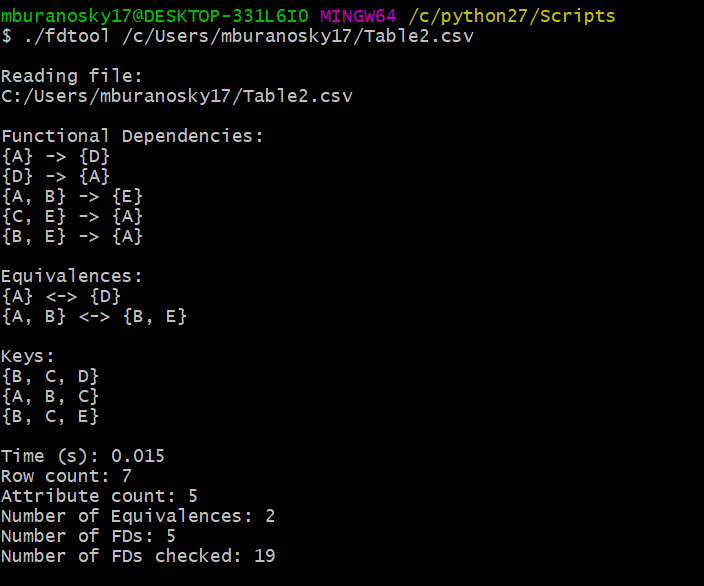
\includegraphics[width=0.95\columnwidth]{sampleOutput}
	\textbf{\label{Fig. 3}}
	\caption{Printed output of FDTool.}
	\label{fig:output}
\end{figure}

\subsection[Implementation]{Implementation}

FDTool is a Python based re-implemntation of the FD\_Mine algorithm. FD\_Mine was published in two papers with more detail given to the scientific concepts used in algorithms of its kind  \cite{fdmine1} \cite{fdmine2}. Yao at al. released two versions of FD\_Mine with different structures but making use of the same theoretical concepts. Their work is fully justified in mathematical proofs of the pruning rules used \cite{fdmine2}. FDTool was coded with special attention given to the pseudo-code in the second version of FD\_Mine \cite{fdmine2}. \footnote{FDTool was tested regularly throughout implementation so as to accomodate changes made to improve runtime and memory behavior.}

The Python script \texttt{dbschema.py} in \texttt{FDTool/fdtool/modules/dbschema} is borrowed from \textit{dbschemacmd} (\url{https://www.elstel.org/database/dbschemacmd.html.en}): a tool for database schema normalization working on functional dependencies. It is used to take well-formatted sets of FDs and infer candidate keys from them. This is explained in \texttt{FDTool/fdtool/modules/dbschema/Docs}.

\subsection[Software availability]{Software availability}

\begin{enumerate}
	\item FDTool is available from the Python Package Index (PyPi; \url{https://pypi.python.org}) via: pip install fdtool.
	\item Latest source code: \url{https://github.com/USEPA/FDTool.git}.
	\item License: CC0 $1.0$ Universal (\url{https://creativecommons.org/publicdomain/zero/1.0/legalcode}). Module \texttt{FDTool/fdtool/modules/dbschema} released under C-FSL license and copyright held by Elmar Stellnberger.
	\item Dependencies: 
	\begin{enumerate}
		\item Python$2$ (\url{https://www.python.org/}), recommended version $2.7.14$ or later.
		\item Pandas data analysis library (\url{https://pandas.pydata.org/}).
	\end{enumerate}
\end{enumerate}

\subsection[Future development]{Future development}

We want to improve its performance so that FDTool is better equipped to handle datasets of different shapes. Using the dependency induction algorithm FDEP, the reach of FDTool could potentially be extended to datasets with more than $100$ columns \cite{expAlgs}. This might also require upgrading the source code with multicore processing methods, such as a Java API, to reduce runtime and avoid reaching memory limit ($256$ GB).

Another goal is to increase the functionality provided by FDTool. This would mean implementing the pen and paper methods typically used to normalize relational schema and decompose tables. Our intent is to incorporate these changes in newer versions of FDTool, released at regular periods, so as to develop it as Python software that could automate much of what is done in the database design process.

\end{section}


\bibliography{myBib}
\bibliographystyle{ieeetr}



\end{document}